\documentclass[conference]{IEEEtran}
%\documentclass[twocolumn]{article}
\usepackage[utf8]{inputenc}
\usepackage{times}
\usepackage{xcolor}
\usepackage{blindtext}
\usepackage{graphicx}
\frenchspacing  
\usepackage{wrapfig}
\usepackage{tabularx}
    
\begin{document}

\title{A Survey on Interest Flooding Attack (IFA) Countermeasures and Mitigation in Named Data Networking (NDN)}

\author{Abdullah Abumouzah\\
College of Engineering and Computer Science\\
University of Colorado at Colorado Springs\\
Colorado Springs, CO 80922\\
Email: aabumouz@uccs.edu}

\maketitle

\begin{abstract}
Today's internet is exposed to a lot of security breaches; one of them is denial-of-service (DoS) or distributed DoS (DDoS). Named-data networking is one of the proposed architectures that promised to resolve many of today's internet limitations, including security weaknesses and vulnerabilities. NDN however is like any other architecture, has its own weaknesses and vulnerabilities. \textit{Interest flooding attack} is one of these attacks that can targeted in the NDN. It could exhaust the nodes resources in the NDN routers or producer's content. This survey illustrates the different ways of how to launch this attack and what are the proposed mitigation and countermeasures including the previous and most recent work.   

\end{abstract}

\begin{IEEEkeywords}
Information-centric networking, Named-data networking, Interest flooding attack, Denial-of-service
\end{IEEEkeywords}

%\nocite{*}
\section{Introduction}
Information-Centring-Networking is considered to be the next future internet architecture \cite{6231276}. NDN is one instance of five projects that funded by the United State National Science Foundation (NSF) under the Future Internet Architecture Program (FIA).

The early revolution of the internet has evolved the concept of the host-to-host communication using the IP address as a presenter for each host. However, with the vast extension of the internet adoption and the need for robust security, users’ requirements and the nature of the applications dispute the capability of current architecture. Thus, there has been a consensus that there is a necessity to develop a different model that address all those services and can concurrently operate on the existing mediums, if possible.  

NDN took its principle from the Content-Centric Network (CCN) architecture that was publically presented in 2009 by professor Van Jacobson \cite{Jacobson:2009:NNC:1658939.1658941}\cite{Jacobson2012}\cite{Fukuda2009}. CCN was created based on the concept of the Host-Centric networking that is used on the current internet; by replacing the dependency of the IP address into the content-name on routing. NDN provides more efficiency and security assurance when sharing data over the public network. NDN abandoned the hosting entity, where users can be more concerned about data than the host of that data per se. Table \ref{tab1} explains the major differences between the host-centric and named-based networking \cite{Abdallah2015}. 

Current internet has been always suffering on security, leaving many threats unsolved properly \cite{Smetters2009}. One of these threats is the DDoS attack. Attackers, using online zombies or bots, can target a specific node or network and exhaust it with a fake packets that causes undesirable traffic. DDoS by overwhelming the network could cause a degradation on the network performance. Furthermore, it could target a specific host which could crash the CPU and shout the service down \cite{6496396}.

\begin{table}[htbp]
\caption{Differences between Host-Centric and Named-Based Networking}
\begin{center}
\begin{tabular}{|c|p{3cm}|p{3.5cm}|}
\hline
{}&\textbf{\textit{Host-Centric}}& \textbf{\textit{Named-Based}} \\
\hline
{Naming}& define host topology position & define content regardless of its location or representation \\
\hline
{Routing}& between hosts using IP address & using name resolution entity or name-based routing  \\
\hline
{Caching}& specific caching points (cache servers) & each node can cache any content passing through it   \\
\hline
{Security}& secure communication channels between hosts & secure the content itself   \\
\hline
{API}& send data to specific address & publish and subscribe contents  \\
\hline
\end{tabular}
\label{tab1}
\end{center}
\end{table}



Although NDN provides a resilient security architecture, DDoS attacks are still applicable. Interests are recorded in the NDN through the router's Pending Interest Tables (PIT) \cite{Cheng2012}. PITs creates new entry for each interest that has no corresponding content on the Content Store (CS), and was not previously requested by another node. Routers use the PITs entries to forward back, at the same path, the retrieved data to the consumer/requester. Attackers can launch a DDoS attack on the NDN by injecting spoofed interests that would neither be satisfied in the routers nor on the end-hosts. Those spoofed interests can either overload the PIT entries in a router which eliminate the ability of the router to serve any further legitimate interest. Also, this attack can be achieved by creating an non-existing interest that would be forwarded to all neighbored nodes all over the internet by the Forwarding Information Table (FIB) \cite{Xin2016ANI}; this approach with an excessive number of spoofed interest could cause a degradation on the network performance. This type of attacks is named Interest Flooding Attack (IFA) in the named data networking. 

in this paper, we illustrates the NDN architecture in section II. Section III explains the IFA attack. Section IV analyze the current literature. Section V provide some discussion questions. in section VI we conclude this paper.   


\section{NDN Architecture Overview}
The principle and sturdy design of the NDN architecture is a derivation from the current host-centric network architecture (IP). \cite{Pan2011}. The phenomenal design of the IP internet hourglass involves the thin waist layer which allows both the upper and lower layers to operate independently; it is however the element that causes most of the limitations of the design per se. IP architecture proposed to allow a communication network among endpoints entities that their packets could only be named digitally through the IP address. However, With the dominant growth of the digital media, e-commerce and social network there became a need to use the internet not only for network communication but for content distribution. As per Cisco white paper \cite{Cisco2015}, on 2014, the content delivery network such as Netflix, Youtube and Akamai had carried about 39\% of the global internet traffic expecting this number to grow up to 62\% on 2019.

Just because how the distribution network is more general than the communication network, it is more complex to solve distribution problems with the IP architecture proposals. NDN hourglass architecture Figure.[1] retains the internet hourglass with evolving the thin waist layer to not only containing those problems, but also providing secured and more efficient platform.

NDN architecture removes the restrictions of using the endpoints as the only source to fetch or secure data. In contrast to the communication network, NDN changes the concept of relying on network services from only delivering the packets from a given node address to also being able to retrieve data that identified by a given name. Thus it serves the content distribution schemes more properly.
\begin{figure} [ht]
    \centering
    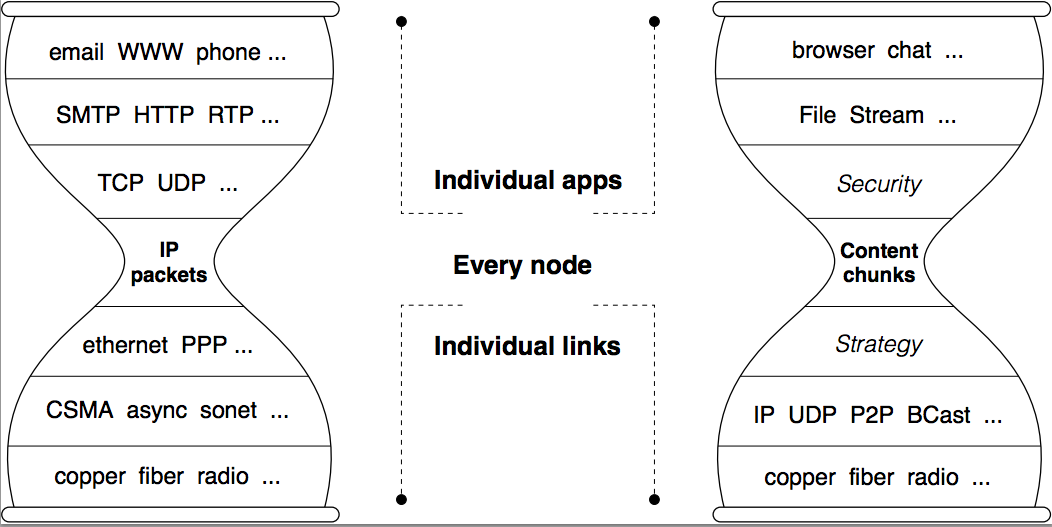
\includegraphics[width=\columnwidth]{hourglass.png}
    \caption{ \small NDN Hourglass Architecture}
    \label{fig:my_label}
\end{figure}

NDN by its mean contains significant components that are used for communication: \textbf{\textit{Interest}} the packet that consumer creates to request a specific content. \textbf{\textit{Data}} the packet that forwards the requested content. \textbf{\textit{Consumer/Requester}} the one that creates an interest packet for a specific content. \textbf{\textit{Producer}} the node that generates and owns the actual content. \textbf{\textit{Provider}}: the node that has a cached content and participates on satisfying the incoming interests. Before the producer returns a requested Data, it gets encrypted and signed by the producer, of which verified by the consumer. 


In order to forward a packet, NDN constructs three structures\cite{Zhang:2014:NDN:2656877.2656887}: \textbf{Content Store (CS)} It caches the arrived Data packets for the future interests that request the same content. \textbf{Pending Interest Tables (PIT)} It contains tables for the pending interests. It Creates an entry for each Interest packet that records the name of the interest, incoming interface and outgoing interface. Once a data packet arrives, router forwards that packet downstream to the requester; if no data packet arrives then the entry expires. \textbf{Forwarding Information Base (FIB)} It is similar to the IP FIBs, which contains a list of the next and available destinations prefix names that forwards the interest packet upstream. Except that IP FIBs rout to the best single next-hop, whereas NDN FIBs route to a ranked list of routes.\\
When a consumer creates an interest packet, the router first searches the CS looking for a matching \textit{Content Namespace (CN)} that associated with the interest's CN; if a match found, a data packet that has the content and was signed by the provider get forwarded to the consumer. Otherwise, the router looks up in the PIT to find a corresponding entry. If a corresponding entry is found, then it creates a new interface for the incoming interest packet and adds it into the interfaces list within this existing entry, which is known as \textit{interest aggregation}. Whenever the corresponding data packet is available, it forwards it to all the consumers that waiting for the data in that entry. If no corresponding entry is found, the router creates a new PIT entry and then forwards the interest packet to FIB. FIB then forwards the interest packet to all the neighbors on the list, where the \textit{longest prefix match (LPM)} is performed for the CN. FIB creates multiple LPMs for the CN. For example, for /youtube/video/CS6000/lectures CN, the LPMs will be like: /youtube/, /youtube/video/, /youtube/video/CS6000, /youtube/video/CS6000/lectures. The forward slash "/" is used to explicitly delimit the boundaries for each packet; it splits the content into segments with predictable and readable names. Once the longest matching found for these LPMs, FIB forwards the interest packet to the next associated hops. Otherwise, the interest packet is flooded and forwarded to all the outgoing interfaces or deleted as per the router's forwarding policies.

When interest packet is satisfied with a data packet, data packet will be returned with the requested content and the producer's key. Figure [2]. When the data packet arrives at the NDN router, the router first looks-up for all the corresponding PIT entries and forwards it, in revers through the same path, to all the interfaces on the list of incoming interfaces related to this packet. Next, router deletes the PIT entry. In the CS, to serve future requests for the same content, the router caches the content based on the local caching policies. 

Because of the lifetime policy of the PIT entry, if the interest packet is not served in a certain amount of time, the PIT entry will be deleted from the incoming list. Accordingly, in case of no corresponding PIT entry is found, the data packet will be dropped too.

\begin{figure} [ht]
    \centering
    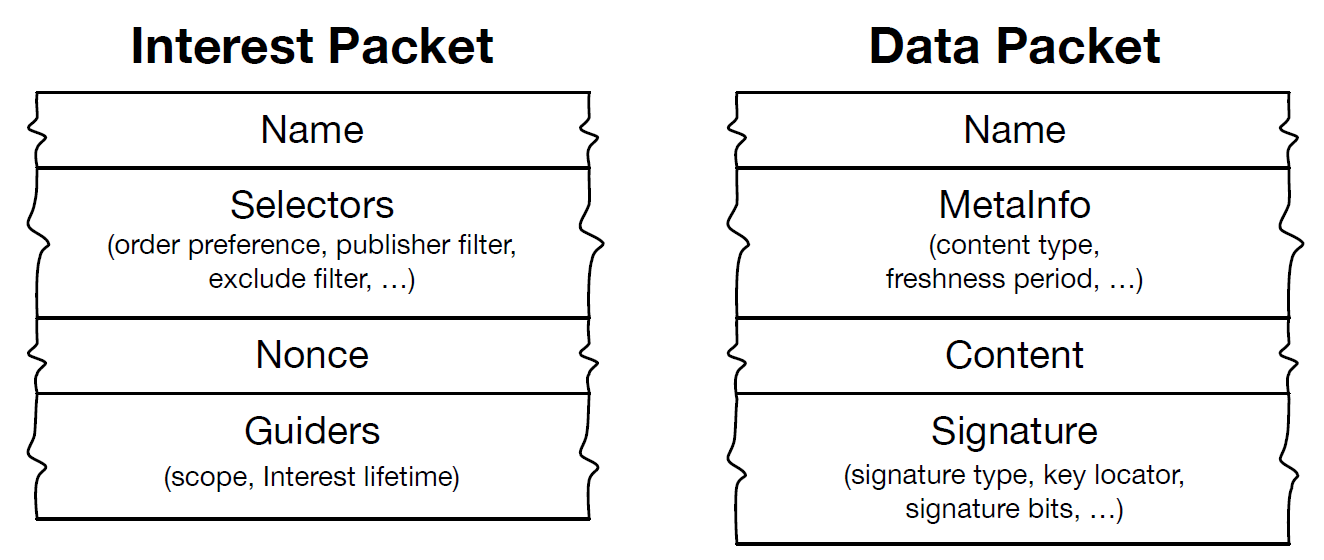
\includegraphics[width=\columnwidth]{NDN_Packets.png}
    \caption{\small Packets architecture in NDN}
    \label{fig:my_label1}
\end{figure}
  
Security in NDN is different from the current host-centric networking. Security is provided in the current internet by securing the mediums, where data and packets are transmitted. It focuses on securing the channels with different security schemes and protocols such as \cite{NGUYEN201517}\cite{661700}\cite{Fumy1998}\cite{Prentice-Hall:2000:ISP:518066}, leaving the actual packets unsecured. Within the growth of network communications, there have been needs to create more protocols to support and serve answering these communications. However, more protocols means more overhead on the network, more standardization, more configuration and less interoperability \cite{cholez:hal-00785298}. Cryptography is one of the proposed solutions that provides a solid security, however, it also adds more overhead on the current processing. In addition, it's not a mandatory feature on a lot of systems that operate on the current host-centric networks.

In contrast, security in NDN concentrate more on securing the data packets than the channels. Contents can be located and retrieved on and from the endpoint hosts as well as the routers. NDN adapts encryption schemes for a robust security. It enforces the encryption at the production stage. Producers are compelled to sign each content with their own digital signature. Moreover, NDN provides a separate layer to encrypt every content; making this scheme a mandatory for all contents which then efficiently guarantees the integrity and authenticity for these packets regardless of how, when or where they are retrieved from \cite{Gasti2013}. Without a need for a digital certificate, NDN facilitates the security implementation by allowing the applications to manage how security is going to be executed and performed.     

   



\section{Interest Forwarding Attack (IFA)}

As previously explained, rather than a specific host’s IP address, NDN routers route the interest packets through the network based on the content name prefixes. When an interest is created, it does not get signed by the consumer; only data packets are signed\cite{Gasti2013}. Once a router receives the interest packet it checks its CS for any existing matched data, if not then it creates a new PIT entry and then forwards the packet to upstream. This make them potential targets for an adversary to inject them with a large imprudent number of malicious interests. Using a large set of zombies on the network, an adversary can mount an excessive number of interests to overflow the PIT in the router which then interdict them to process legitimate interests. In addition, producer's content can be targeted too by swamping the content at the producer's end which then overwhelm the producer with the demanding requests computation. However, attackers cannot target a specific host. Instead, they can target a specific namespace regardless of where or which endpoints host the content. Intermediate routers also consume their memory when serving an interest packet. Therefore, not only endpoints are effected, but also the intermediate routers could be targeted too for such attack \cite{6663516}\cite{KARAMI20151262}. Figure [3] shows how a legitimate user could only receive back one data packet only for four interests. This figure shows that the attackers inundate PITs with spoofed interests which prevent the legitimate interests to be served and dropped throughout the network.  

\begin{figure} [ht]
    \centering
    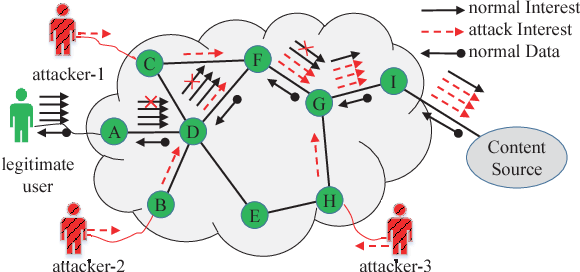
\includegraphics[width=\columnwidth]{IFA.png}
    \caption{\small Interest Flooding Attack  \cite{Xin2016ANI} }
    \label{fig:my_label2}
\end{figure}

As noted on \cite{Gasti2013}, Interest flooding attack is classified into three different categories based on the type of requested content: 
\begin{enumerate}

        \item Existing/Static Content: What impacted in this attack is the network infrastructure. Since the content is cached and exists in the CS of the router (in-network content caching), malicious interests that created to target a producer will be satisfied at the routers that have these cached content; and will not be propagated to the producer. Therefore, the the countermeasure is built-in and the impact is narrowed.  
        \item Dynamically Generated Content: What impacted in this attack are both network and content producer. In this type of attacks the built-in content feature is not helping as the content is dynamic which means that the attacker periodically initiates malicious interests from different routers. Therefore, the generated interests will be forwarded to the producer. thus consuming the bandwidth will at the high level of the network infrastructure. Also, as large the malicious interests could be that will exhaust the router's PITs entry. For this, the closer the routers to the producer, the larger impact they will gain. In addition, as much of the illegitimate interest the producer receive that will prevent the legitimate interests to be served.        
        \item Non-Existing Content: What impacted in this attack is network infrastructure and resources. Attackers here create interests that not exist therefore they can not be satisfied. Once a router receives such interest, it forwards it to upstream trying to deliver it the producer. This interest will be forwarded until it reaches the edge of the network where it will pending to be either satisfied or dropped due the expiration policy. If zombies create an excessive amount of such interests, that will harm the network infrastructure and the network resources including the bandwidth and the intermediate devices that participate on processing.          


\end{enumerate}


\section{Analysis And Current Literature}
A naive solution for the IFA attack is to prevent the proliferation of the malicious interests throughout the internet. However, such countermeasure is not applicable on all cases. To mitigate this attack, the current published literature focused on most of the components that might cause such attack. However, there are still possible solutions that could be applied. This survey focus on three mitigation monitoring categories which mostly play core roles on this attack. In general, router can monitor the state of an interest as well as the PIT's size; by doing so, router will be able to decide the abnormality behavior of the interest and decide to either keep it, eliminate it or delete it.   

\subsection{Per interface Monitoring: }
NDN routers keep monitoring the flow of the interests. Mostly, for an interest flows upstream there should be one content flow downstream that can satisfy this interest. Therefore, the router should be able to compute and monitor the rate of pending number of interests for each outgoing interface that downstream can satisfy prior to their time-out ration. In addition, As per the limitation of the physical downstream link, the router should be able to notice when an excessive number of interests is sent by the downstream that therefore can not be satisfied. By that, the router can easily detect the IFA attack which then can mitigate it by controlling the flow rate of the malicious interests. 

Gasti \textit{et al}. \cite{Gasti2013} analyzed and explored the DDoS attack concentrating more on the NDN interest flooding attack. their analysis addressed attack based on the type of the requested content, either the attack is launched requesting (1) existing/static content, (2) dynamic generated content or (3) non-existing content. 

To mitigate this attack, authors proposal was to monitor and maintain the flow balance of the interests. In this approach, the router can track the number of pending interests for each outgoing face. Also track the number of unsatisfied interests for each incoming face. Once a threshold is exceeded, routers can control and limit the number of these pending and unsatisfied interests which eliminate the suspicious interests.  

Afanasyev \textit{et al}. \cite{6663516} proposed three different approaches that mitigate the interest flooding attack. first proposal was a model named \textit{Vanilla model}, which is a modified version of the IP based model known as \textit{Token Bucket}. This approach proposed an augmentation of the vanilla model with the concept of fairness for each interface. With this concept the Uplink capacity will be proportionally shared for the outgoing interfaces and incoming interfaces. Router can limit and control the number of upstream forwarded interests based on the number of pending interests (fairness use of the bandwidth). Therefore, if there is a large number of pending interests, newly arrived interests will be dropped. One thing this approach can not distinguish is the source of interest, if it is from  legitimate or attacker user.thus the bandwidth could be consumed by attacker's interests instead; and the legitimate interests are dropped accordingly.

The second proposed approach is to calculate the ration of the interest satisfaction with the number of forwarded interests which create a satisfaction-ratio. Router can provide an interface with higher rate of satisfaction a higher share of the outgoing capacity of the link. However, Paths with great have length have the possibility to face congest ions which increase the number of dropped interest. This will allow the router to decide if it is possible to forward interests and when should to avoid incoming content. 

the last approach is based on the satisfaction-ration too. As each router will be able to calculate its own limit number of incoming interests based on the satisfaction ration,  Authors suggested that routers can also announce their satisfaction ratio to their downstream neighbors who then should reconfigure their own interests limits of acceptance accordingly to what the upstream announced.     

Compagno \textit{et al}. \cite{Compagno2013} proposed a framework named Poseidon that targets the non-existing type of content. Their design was a collaborative scheme to mitigate the interest flooding attack involving a detection phase and a reaction phase. Withing the detection phase, the collaborative mitigation is executed when the threshold is met. The detection is carried out at the router which depends on two values based on a time window: the calculated ration of the outgoing content to the incoming interests; in addition to the PIT size that consumed by an interface. Once a threshold is met, router adjust its rate limits and also send a notification for the downstream informing them about the attack. Downstream routers then can reconfigure their rate limits as well. 

Routers reduce the PIT size as a reaction of the attack. However, this reduce the interests satisfaction rate. Therefore, Authors noted that notification approach is more effective than reducing the PIT size approach.

The countermeasure scheme was simulated on a small attack model, and it was noted that about 80\% - 90\% of the bandwidth was available during the attack.       





\subsection{PIT Size Monitoring:}

Routers can benefit from monitoring the Pending Interest Table (PIT) size state. A threshold can be set to monitor the growth of the PIT size that once it is met the mitigation phase can be performed.  

Dai \textit{et al}. \cite{Dai2013MitigateDA} designed a scheme that was stimulated from the IP-traceback approach to mitigate the interest flooding attack. Using this scheme, routers can trace back the originator of the malicious interests. this approach is performed once the PIT size exceeds the threshold. This scheme sends spoofed data packets to satisfy the longest unsatisfied interests; by doing that, it reaches the edge of that attacker and notify it with the suspicious behaviour which then it rate-limits that attacker's interface as a response.   

This approach might also treat the legitimate interests with the same reaction. If a legitimate user sends a non-existing content it might be rate-limited as a response if the PIT size met the threshold by attacker's interests. Also, in case the edge router itself is compromised this mechanism will be ineffective.     

Lixia \textit{et al.} \cite{Zhao2018} proposed a sophisticated scenario of the interest flooding attack. In most of the proposed studies, authors analyzed the attack as a huge number of malicious interests are injected into the intermediate routers. 
In their scenario, the attacker sends a low rate of malicious interests at the beginning to circumvent the abnormality state of the PIT entries size; and to make sure that the PIT size is always under the normal level. Gradually, the attacker increases the rate of the malicious interests trying to exhaust the victim's PIT. Whereas, the intermediate router that near to the attackers will not recognize the attack due to the unnoticeable information state changes between the two sequential intervals.

To mitigate this attack, authors proposed a potential central controller mechanism. The central controller monitors all the nodes on the network as well as the status of the network in general. It make decisions based on the shared information from all nodes. If a router notice abnormality behaviour of the PIT seize increasing over a period of time but no increasing on the number of PIT sizes, and it is not sure if that is related to an attack, it sends these information to the controller. The controller then, based on the overall state of the network decides if there is an attack or not. In case of an attack, the controller alerts only routers that close and related to the attack require them to perform the right countermeasures to prevent the attack. 
   



\subsection{Statistical monitoring:}

This approach depends on monitoring and identifying the abnormal behaviour of the traffic flow based on the statistical information on the router's PIT and interfaces. 

Wang \textit{et al.} \cite{Wang2014} proposed an architecture that called Cooperative-Filtering. The scheme is built upon the cooperation between fuzzy logic and routers providing a detection and mitigation mechanisms against the interest flooding attack. Fuzzy logic is used, using a cooperative-filtering, to estimate the possibility of the IFA attack. The mitigation is performed by the cooperation between routers. Cooperative-Filtering tend to catch the attack at every router in the network but mitigate it at the edge routers of the attacker; To do that, it consolidate the Logic Fuzzy based on two mechanisms: First is the Detection Mechanism, which periodically monitors the PIT occupancy rate (POR) and  PIT expiration rate (PET). "(POR) calculates the temporal number of PIT entries ration against the maximum number of PIT entries in real life"; where as, "(PER) represents the number of expired PIT entries ratio against the the total number of PIT entries in real life". Fuzzy interface rule use the collected POR and PER in real time to determine of their state if normal or abnormal. Second is the Mitigation Mechanism, which enable the push-back scheme, once an abnormal state of either POR or PER is detected, to first trigger and apply a rate control for this specific interface, then notify the downstream routers that related to the attacker's edge to reset the limit rate on their PIT and eliminate the number of malicious interests.

This approach proofed its effectiveness for reducing the consumption of the PIT memory as well as increasing the rate of of the legitimate interests satisfaction. However, since it only triggers and monitors the attacker's prefixes the mitigation is effective to prevent attacks that target a specific publisher but not attacks that target the network infrastructure. In addition, the DDOS attack is still applicable.    

Nguyen \textit{et al.} \cite{Nguyen2015} proposed a scheme to detect the interest flooding attack that is based on statistical hypothesis testing theory. Their proposed detector strengths lay on three features: (1) The scalability; (2) controlability of the false alarm and (3) analytically established evaluation. The scheme is simply designed to monitor the rate of interfaces with and without the attack. The ratio of the interfaces when there is an attack is higher than the ratio in normal conditions. Meanwhile, the rate of data retrieved remains the same in both hypotheses. As a result, the data ratio under attack comparing with the normal conditions is lower. Authors in this scheme rely on the false-alarm controlability to determine when an attack is occurring by resetting the detection threshold accordingly \cite{8452848}.    

To evaluate their hypotheses, they implement their scheme in a simulator with only one attacker and eight nodes, which bounded the effectiveness evaluation on a bigger topology or when there is a distributed ddos attack.

Vassilios \textit{et al}.\cite{Vassilakis2015} proposed an approach that mitigates the interests flooding attack upon the user behaviour, which improves the detection ability at the early stages of the attack. Their approach classified routers into two types: One type is the \textit{Edge router} which is connected directly to one or more users. This Type provide an additional security layer by detecting any abnormal user's behaviour and notify other routers about it. The other type is \textit{Core router}, which is connected directly to the other routers or sources. This Type provide the attack notifications and share them with all other routers among the network. Authors proposed three phases of the mitigation mechanisms: First phase is the Attack Detection where the edge router detects the abnormal behaviour of the user and then identifies this user as a suspicious or an attacker. Second phase is Rate Deduction or Blocking, where the edge router starts reducing and limiting the data rate for the suspicious user and block the attackers. Third phase is the Attack Notification, where the edge router starts notifying the other routers in the network about the deducted attack and the identity of the suspicious users which prevent the dynamic/mobile interests flooding attack.


To improve their scheme and to empower the notification phase effectively, they proposed a public-key based scheme that allow only the authenticated routers to share those notifications which then protect the network from the any malicious notifications. This scheme is based on the Certificate Authority, where routers that directly connected to the CA can be trusted. Whereas, router that no directly connected to the CA must at least be authenticated by a mediator, a router that directly connected to the CA, in order to be able to share a notification.      





\section{Discussions}

In spite of the fact that there are plenty of contributions to mitigate or eliminate the impact of the interests flooding attack but the attack is still attainable. However, it does not mean that the proposed solutions were not feasible, but the attack aspects are myriad and stressful. Most of the proposed mechanisms impacted the legitimate interests in a way or another. The drawback of the rate limiting based solutions, for example, that was supposed to countermeasure the suspicious interfaces could penalize the legitimate user's interests and limit its rate ration.   
 
In addition to the aforementioned papers, there are other mechanisms, not covered in this survey, that mitigate the attack from different aspects. One of which that proposed to modify the router's components by increasing and augmenting the router with a bigger PIT, longer caching time and delete the malicious interests from the router's PIT \cite{Wang2012}\cite{Virgilio2013}. Other approaches proposed solutions with a proof of the client's work\cite{Li2014}. However, most of those were reactive not proactive approaches. Meaning that, they might detect the attack by monitoring the interface and PITs size then mitigate it by limiting or eliminating the malicious interests.  

Using the Stateful protocol, which enable the the interest and data exchange, provides some benefits to the NDN architecture. One benefit is that PIT maintains the forwarding state of the interest/data, enabling the router to monitor and forward a content back and forth easily by identifying the interface that corresponding to the PIT entry. In addition, PIT uses the entries mechanism that allows to create an entry for a new received interest, however, if there is a related entry to that interest it shall be added to this entry which avoid the redundancy of the PIT entries in the router. Also, by exchanging the information about the Round Trip Time (RTT) of the interest and content, PIT can provide a good balance of the network path to avoid congestion \cite{Yi2012}\cite{Wang2013}. 

With all the aforementioned facts about PIT, attackers can easily exploit its resources to launch the IFA attack by exhausting the PIT memory on a router or degrading the network performance by proliferating the number of malicious interests. Therefore, in such cases, router will either drop the new incoming interests or delete existing entries to free some resources for the arriving interests. However, again that might also affect the legitimate interests.     

There are alternative contributions to proactively mitigate this attack. 

Another way to deal with this attack is to be proactive. There are some other contributions covered the attack's  


\cite{Ghali2015}


Most of the proposed works are reactive not proactive 

\cite{Chen2015}
\cite{Ahlgren2012}
\cite{Universite2018}

\cite{Tourani2018}
\cite{Bhattacharyya2018}
\cite{Chhetry2016}

\cite{8352953}
\cite{8247232}

\cite{Xin2016ANI}
\cite{Zhang:2014:NDN:2656877.2656887}
\cite{Compagno2013}



\cite{Abdallah2015} 
\cite{Zhao2018}


    I should cover the other type of threats that target NDN security. 
    item Attack that targets the CS.
    item Since CS and PIT are the two structures where mostly consume the memory when serving an interest packet, they are potential for the IFA attack. 
    item Attack that targets the FIB 

\section{Conclusion}




\bibliographystyle{ieeetr}
\bibliography{Bibliography}
\end{document}
